En esta iteracion se implemento la opcion de anadir mas lugares al sistema, de editarlos y eliminarlos, y la primera tarea es crear las consultas SQL para llevar a cambo las tareas. \\

% por lo que es necesario crear las consultas SQL que insertaran los datos enviados desde el dispositivo movil al servidor. \\

Como requisito para insertar un nuevo ``lugar'', se requiere que el usuario este posicionado en el ``lugar'' ya que se usaran sus coordenadas para posicionar el ``lugar''. Las coordenadas del usuario son obtenidas usuando el API de Geolocalizion propia de HTML5, usada anteriormente para encontrar la ubicacion del usuario \emph{visitante} en la iteracion 2.\\

Posteriormente se necesita implementar el formulario que el usuario usara para insertar los datos del ``lugar'': el nombre, la descripcion, el telefono y el nivel.\\

Para insertar un ``lugar''  en la base de datos se uso el codigo \ref{new_place}, donde se puede observar la consulta SQL usada, para la cual se necesita capturar la latitud y longitud respectiva donde se encuentra el usuario, ademas de los datos del ``lugar''.\\

\begin{center}
  \begin{lstlisting}[label=new_place,caption=Insertar un ``lugar'' en la base de datos.]

    var newPlace = (req, res) => {
        var name = req.body.name || '';
        var lat = req.body.lat || '';
        var lon = req.body.lon || '';
        var description = req.body.description || '';
        var phone = req.body.phone || '';
        var level = req.body.level || '';

        let raw = `insert into place (name, geom, description, phone, level)
                   values ('${name}',
                           ST_GeomFromText('POINT(${lon} ${lat})', 3875),
                           '${description}',
                           '${phone}',
                           '${level}'
                          );`;

        Knex.raw(raw)
            .then(function(data) {
                res.json({
                    "message": "Place saved successfully!",
                    "data": data
                });
            })
            .catch(function(error) {
                res.send("Error: ", error);
            });
    };

  \end{lstlisting}
\end{center}


% Para la creacion de un ``lugar'' es necesario implementar un \emph{endpoint} en el API y siguiendo las convenciones REST se , para que como ya se explico anteriormente el frontend pueda comunicarse con el backend. \\

En el API de la aplicacion, se implemento un \emph{endpoint} para que pueda manejar los \emph{request} del cliente para añadir un lugar, este \emph{request} es enviado usando el verbo HTTP \emph{POST}, que como ya se explico es el usado en un REST API para crear objectos. \\


\begin{figure}[H]
      \begin{center}
        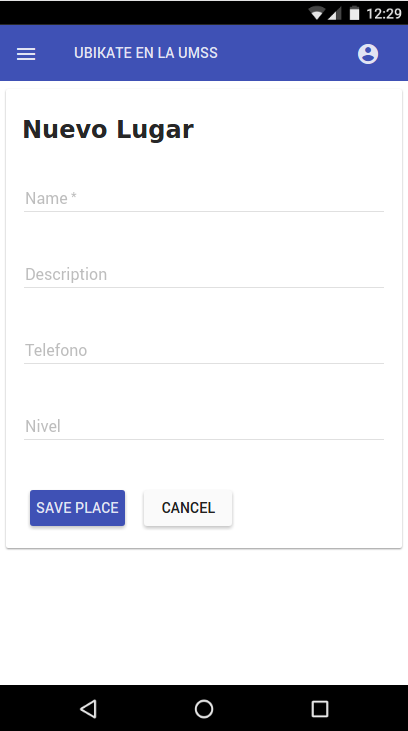
\includegraphics[width=0.3\textwidth]{new_place}

        \caption{ Formulario para anadir un nuevo ``lugar''}
        \label{fig:new_place}
        \caption*{Fuente: Elaboración propia.}
      \end{center}
\end{figure}

En la figura \ref{fig:new_place} se puede ver el formulario implementado usando \emph{ember-paper}, el cual coleciona los datos que se quieren introducir y se los envia al backend usando una llamanda AJAX, como se puede ver en el siguiente codigo, para crear la peticion POST se obtiene las coordenadas actuales del dispositvo movil ademas de los datos recolectados del formulario y que con la ayuda de \emph{JQuery} es enviado al API el cual maneja la informacion recibida y se encarga de insertar los datos en la base de datos.\\


%
\begin{center}
  \begin{lstlisting}[label=new_place_request,caption=POST request creado en el controlador de \emph{ember}]

    var payload = {
        name: nombre,
        description: descripcion,
        phone: telefono,
        level: nivel,
        lat: latitud,
        lon: longitud
    };

    var url = (ENV.APP.API_HOST || '') + '/api/v1/places/';
    jQuery.post(url, payload).then(
        function(data) {
            var transition = controller.get('transition');
            if (transition) {
                self.transitionTo('places.show');
            } else {
                self.transitionTo('places');
            }
        },
        function(error) {
            controller.set('message', error.responseText);
        }
    );

  \end{lstlisting}
\end{center}

Una ves implementado la logica para añadir un ``lugar'', se implemento los modulos para poder eliminar el ``lugar'', para esto se añadio un boton en la lista de lugares, el cual desplega un mensaje de advertencia al usuario de que esta por eliminar un ``lugar'' y que la accion es irreversible, por lo tanto este boton solo esta disponible para un usuario \emph{administrador}. \\

La verbo  HTTP \emph{DELETE} es el que deacuerdo a la implementacion del API REST es el adecuado para eliminar un lugar, por lo tanto es el que se uso en la aplicacion. En el codigo \ref{delete_place_enpoint} se puede observar el \emph{endpoint} implementado en el API que se encarga de manejar las peticiones \emph{DELETE} creando una consulta SQL que elimina el lugar de la base de datos.\\

\begin{center}
  \begin{lstlisting}[label=delete_place_enpoint,caption=DELETE request elimina un lugar.]

    router.delete('/:id', places.deletePlace);

    var deletePlace = (req, res) => {
        var id = req.params.id;

        Place.forge({
            gid: id
        })
        .destroy()
        .then(function(model) {
            res.json({
                "message": "Place deleted successfully!"
            });
        })
        .catch(function(err) {
            res.status(500);
        });
    };

  \end{lstlisting}
\end{center}

En el anterior codigo se puede apreciar la bondad de usar un manejar de bases de datos como \emph{Bookshelf} ya que usando el metodo \verb|destroy()|, se encarga automaticamente de crear la consulta SQL para eliminar una tupla de la base de datos.\\
